\documentclass[paper=a4,twoside=false,BCOR=0mm,DIV=calc,fontsize=12pt]{scrartcl}

\usepackage[automark,headsepline]{scrpage2}
% \usepackage{xunicode,fontspec,xltxtra}
\usepackage[english,german]{babel}

\usepackage[T1]{fontenc}
\usepackage[utf8x]{inputenc}

\usepackage{graphicx}
\usepackage{lastpage}
\usepackage{listings}

%Schöne Tabellen
\usepackage{booktabs}

%\usepackage{longtable}

\usepackage{multirow}

% Kein einrücken und Abstand zwischen Absätzen.
\usepackage{parskip}
\setlength{\parindent}{0cm}

% Hyperlinks und url's
\usepackage[hidelinks]{hyperref}



% \usepackage[debug]{libertine}
% \setromanfont[Mapping=tex-text]{Linux Libertine O}
% \setsansfont[Mapping=tex-text]{Linux Biolinum O}
% \setmonofont[Mapping=tex-text]{Liberation Mono}

\pagestyle{scrheadings}

\clearscrheadfoot
\ihead{\headmark}
\ohead{Seite\pagemark\ von \pageref{LastPage}}
\ifoot{Business frameworks}
\cfoot{{
\includegraphics[width=1.5cm]{./img/CC3.png}}}
\ofoot{\today}

\renewcommand*{\pnumfont}{
	\normalfont\rmfamily\slshape
}

\KOMAoptions{draft=false}
\KOMAoptions{DIV=last}

\begin{document}

% --- Titelseite --- %
\begin{titlepage}
	\enlargethispage{3cm}
	\begin{raggedright}
	\begin{picture}(0,0)
		\put(-30,14){
\includegraphics[width=7cm]{./img/fhnw-technik-head}}
	\end{picture}

	\vspace*{6cm}
	{\Huge\bfseries\sf
		MAS-IT\\[1.7ex]
	}
	{\Large\bfseries\sf
		Business frameworks\\[2.2ex]
	}
	{\large\bfseries\sf
		Masterthesis von\\[1.5ex]
		Etienne Rebetez\\[1.5ex]
	}
	\vspace*{1.5cm}
	{\large\bfseries\sf
		FHNW\\[1.5ex]
		Hochschule für Technik\\[1.5ex]
		Studiengang MAS-IT\\[1.5ex]
		Betreuender Dozent:\\[1.5ex]
		Dr. sc. techn. Ronald Tanner\\[1.5ex]
	}
	\vspace*{2cm}
	{\large\bfseries\sf
		Bern, \today\\
	}
	\end{raggedright}
\end{titlepage}

\newpage
% --- Zusammenfassung --- %
\section*{Summary}
Text

% --- Vorwort --- %
\section*{Vorwort}
Text
% --- Inhaltsverzeichnis --- %
\newpage
	\tableofcontents

% --- Einleitung --- %
\newpage
\section{Introduction}
Laboratory processes. What is that all about?

Usually it goals like this. A physical sample is brought to the quality control (QC) analytic laboratory. The laboratory determines certain physical property's and then tell the customer about it.

A simplified view looks like this. A sample of a certain substance comes into the QC lab. What analysis have to be made etc. is given by the Labor information and management system (LIMS). The LIMS also says when and what sample has to be analyzed.
The lab performs then the analysis. All used solutions, instruments and steps have to be documented. That is traditionally done on paper. At this point it is important to emphasize that everything that is not documented isn't done from an audit point of view. Also the standard operating procedure (SOP) has to be followed exactly.
After the analysis it is mostly used to have a calculation step where certain parameters are calculated to the final value. The final value is then transferred back to the LIMS. These are mainly manual steps. These manual steps can lead to errors and are time consuming.
Since the operating of balances, creation of solution or other practical tasks cannot be automated, the data flow and the process can.

This report aims to look at the layer between LIMS and the instruments and the analysis method. In the past few years there has been a ton of programs that aim to solve that problem. Some try to achieve that with an almighty LIMS. But since most LIMS date from the 90's the implementation is not easy and you end up haven a not maintainable monolith. There was also the idea of electronic lab notebooks (ELN) these ELN where usually conceived for R\&D laboratory. That means more freedom and less strict processes.
Then there is the software for the instruments, that can perform more and more tasks. This looks like a good idea, but there are so many instruments, methods and manufactures that there is just no solution that fits all. Also it is still the case, that one solution of one manufacturer is in no way compatible to the solution of another manufacturer.


\section{The Laboratory landscape}
The laboratory knows many different analytic methods. They all have different requirements and provide different forms of results.
That gives us an extremely heterogeneous landscape. 

% TODO instrument software exkurs. 


First we need to look at the current laboratory work flow, with the given programs. Historically, and still so, the lab uses the LIMS to see what samples have do be done and to type the results back. The LIMS is a height level program that was designed to managed samples.

To normalize the data and provide an easy reviewability every step created a report that can be viewed and signed in the SDMS database.

\begin{figure}
    \begin{center}
      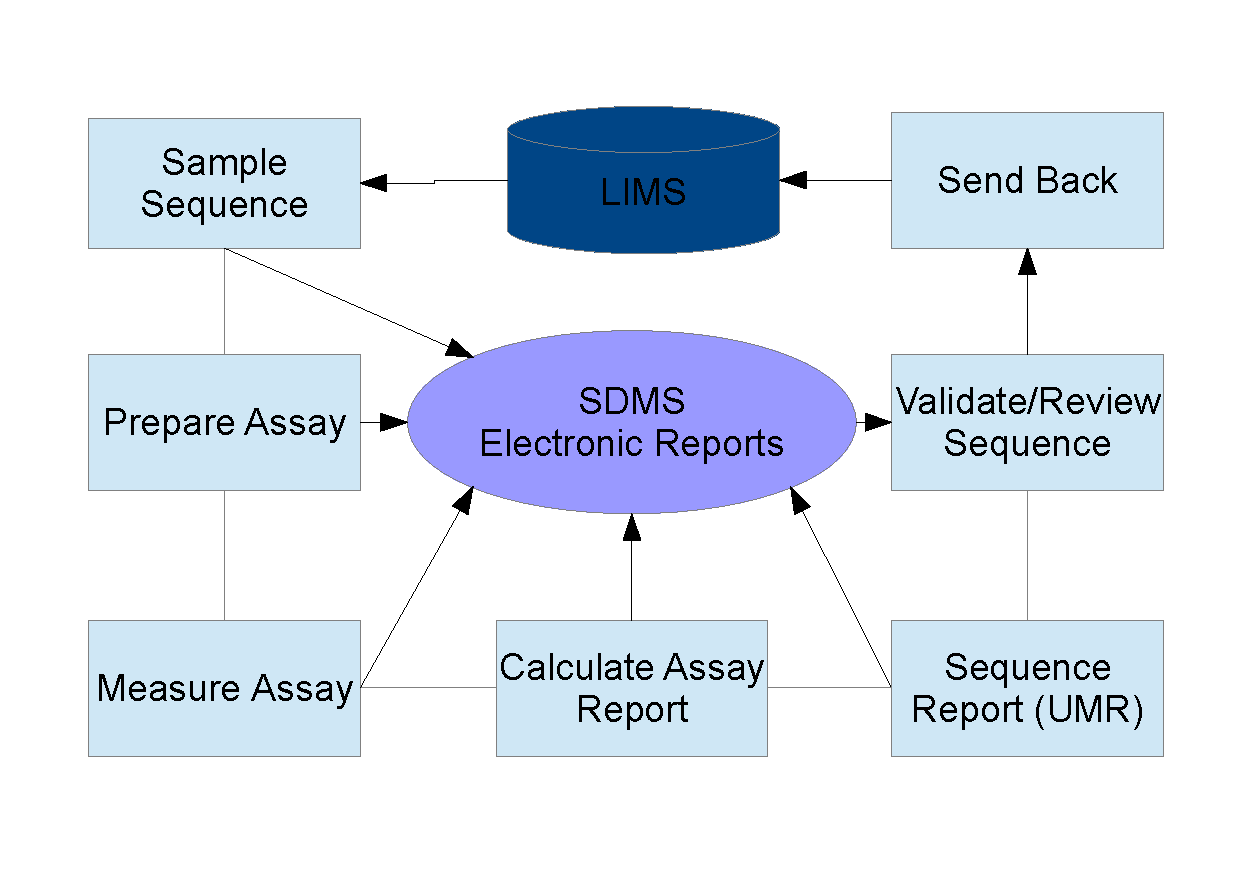
\includegraphics[width=1\textwidth]{./img/Laboverview.eps}\\
    \end{center}
  \caption{The current lab work flow}
  \label{CurrentLabWorkflow}
\end{figure} 




\section{Concept}
So the question came up, why not look at something completely different. The lab is not the only business that has processes. There could be other business frameworks that provide the needed functionality. This system should be able to integrate and interface these different islands of programs. It would be like a laboratory middle ware.

To make the automation in such a heterogeneous landscape possible a sort of state machine is needed. This state machine knows how process
look like, which processes are currently run, in which state they are in and which is the next to execute.
This pattern is basically the same in every business process. One of the therms is SOA (Service Oriented Architecture). The state machine engine would therefore be the heart of the hole automation process.

Since the lab is obviously not the only place in the world that has predefined process a look at generic state machines was imminent.
To configure these state  machine engines there are already several standards. Two process definition languages are already well established:

\begin{itemize}
 \item BPEL
 \item BPMN
\end{itemize}

Both are open standards from OMG \cite{omg}.


\subsection{Requirements}
%FIXME translate ....
Neben dieser Zentralen Steuerungseinheit, soll es dann auch möglich sein, Komponenten wie Webapplikationen (Formulare, Listen, etc),
Reports oder Mobile Geräte einbinden zu können. In den Labors ist es zudem Historisch so, das viele MS Excel Berechnungen existieren. Diese
sollten, dann auch in den Prozessen eingebunden werden können.


\section{BPEL}
The BPEL (Business Process Execution Language) was an answer to the process problem that came from the it world. It is very technical and the process description is made with if's, loops that are also known in common programming languages. 

\section{BPMN}
BPMN (Business Process Model and Notation) has it roots in the business process modulation. It first was only a description language to provide some unified task ore gateway definitions. These are the elements of the common flowcharts.
With the versin 2 of the BPMN standard these flowcharts can now be interpreted by an engines and be run as a program.


\section{Prozess Engines}
The engines are implementations of these business description language. The engines provide all sort of logic that would be hard to implement every time from scratch.
\begin{itemize}
  \item What processes are there
  \item which are in what state
  \item Processes are recoverable and transaction save. (crash)
  \item What happens if a new version of the process is deployed.
  \item Who did what and when.
\end{itemize}


The following chapters present some of these engines that are already available. The list is far from complete.

\subsection{activVOS}
Programmer: Active Endpoints, Inc.

Language: java

License: proprietary (setzt aber auf offenen standards)


Cost?

Dokumentation: Diverse Videos mit Demos und Tutorials.

Remarks: It's basically an eclipse Plugin. \\
Has a report designer. \\
Viele GUI's


\subsection{biztalk}
Hersteller: Microsoft

Sprache: .NET

Lizens: proprietär


Preise?

Dokumentation:

Bemerkungen:
Zusammenspiel mit Sharpoint.
nur für BPEL



\subsection{Apache ODE}
Hersteller: apache fundation

Sprache: java

Lizens: open source (Apache License 2.0 )

Bemerkungen:
Nur BPEL engine



\subsection{activiti}
Hersteller:

Sprache: java

Lizens: opensource (Apache License 2.0 )


Bemerkungen:
Nur BPMN engine
Schlank und aufgeräumt. 
Relativ neu aber Fork aus jBPM.


\subsection{ARIS}
Hersteller: software AG

Sprache: java

Lizens: proprietär

Preis?

Bemerkungen:
Unterstützt BPMN und BPEL. (xml nicht sichtbar/exportierbar...)
Viele GUI's. 
Monitoring, Reporting werkzeuge dabei.
Hauptsächlich für SAP entwickelt
Wird eventuel von <Firma> eingekauft/verwendet.
Programmierung und Konfiguration muss fast eingekauft werden.



\subsection{Summary of products}
Since either BPMN nor BPEL is in use at the moment the first thing to decide is what specification to use.
It does not make sense to mix both. 

BPMN 2.0 seems to be the better choice due to the close process view. BPEL exists longer but seems unnecessary complicated.
Therefore BPMN is the better choice for the lab process definition. 

If we now only look at the BPMN 2.0 engines only ActiVOS, activiti and ARIS remain from the list.

ActiVOS provides some extra GUI's to give "simpler" access to the configuration. It creates xml and configuratoins in the background.
They can fortunately be seen and changed from hand. In the bottom line, it seems nice but does not provide a big advantage. 

ARIS is the big all inclusive package. It is however impossible to work yourselves on the project they sell also the programming and support. Therefore there is no code ore xml visible in the hole package. So for each change the external company has to be contracted.
They provide also some basic training courses.

Activiti has a total other approach. It has no gui what so ever. I provides an open programming interface that provides all functionality 
of the engine. The xml can be easily edited directly. It is therefore slim and sticks to the one task it tries to solve.
The downside is that there is a steep learning curve since everything has to bee implemented in the code. 
Because it is open source there are already some example web application that can be used out of the box. 

\subsection{Conclusion}
The monolithic concept of big systems has proven in the past to be inflexible and heavy on the maintenance. 
The decision was made to use activiti because of its simplicity and possibility to add other functions (i.e monitoring or reporting) in the future over other programs that also have one functionality.
Activiti plays also well together with the web framework vaadin.


\subsection{Compatibility}
Although BPMN is a standard and provides most keywords and rules the implementations still adds own keywords or extra functionality (i.e
forms). So the BPMN files can't just be copied form one engine to another. If you chose one engine it is kinda final and you will stick to it.

If a engine change really has to be made it is however simpler to achieve than if you had the complete logic inside the code. If the new engines even
uses the same programming language, it is very probable, that you can just reuse the business logic classes. 



\section{Example Application}
The process takes an annual inventory item review. These items are reference samples of the substance that were sold.

\begin{figure}
    \begin{center}
      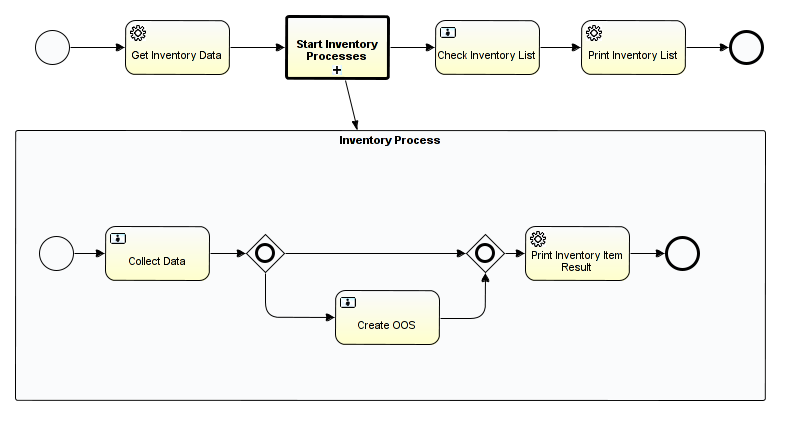
\includegraphics[width=1\textwidth]{./img/PanExampleBPMN.png}\\
    \end{center}
  \caption{Example Application work flow}
  \label{panexampleWorkflow}
\end{figure} 

First a list of the reference samples that have to be checked is retrieved from the parent system (i.e LIMS). This is done with a SQL query on the database. 
The sample number and the location is then stored in a process variable as a data object list.

For each item in the list a sub process is started in parallel (callActiviy). The sub process is a separate bpmn process definition.
The data object which represents a sample, is given to the newly created process.

Now the user can claim the tasks or in this case the samples they wish to check. Then they go to the location and provide the verdict of that sample. If the sample is fine a report is created otherwise a OOS (Out of specification) procedure has to be started first. The OOS process is not part of this demonstration application. It would however be very easy create and to call another sub activity in the future.
To print the reports the existing infrastructure is used. The reports are stored in the SDMS and can be signed there..
Once all samples have been controlled, the parent process goes to the next task.

The laboratory supervisor now gets the task to check the sample list. An overview of the sample list and the verdicts is presented to him.
The list with all samples is then again printed to the SDMS. That concludes the review process.

This process is used to illustrate the further examples and references.



\subsection{Technology and architecture}
Since activiti seems a good choice the main language will be Java.
Java also brings a lot of classes and tools to process xml and other data.


\section{Webapplication}
Besides the bpmn engine, the webapplication is a central cornerstone of this project. After all thats what the user gets to see.
The decisions was made to use Vaadin as a webframework. It allows to program the webapplication completely in java on the server side. So there is no need to get in trouble with webtechnology.

As the back end activiti is used. So the user management, transaction safety and business logic is taken care of.

To glue all the frameworks together, spring is used. In spring the configuration is made in a xml file. As a result the code doesn't has to have any knowledge of the environment it is in.


\subsection{class design}
%TODO class image of app%






\subsection{Internationalisation}




\subsection{ldap}


\section{Extern application server}

The basic concept is a socket client server architecture. 

\subsection{server}

The server receives a request to execute a certain excel application. It then executes this application. If multiple request are received the external excel application are run in a serial way.

%TODO class diagram server.




\subsection{client}

The client is a process on the bpmn engine server. This process can be called by a parent process (see callActiviy). 
The first task is a service task. It creates a connection to the server and sends the data. After that a message task waits for the 
response.

If there is no response in a given time a boundary event is fired and a user or e-mail task is started. When the problem is resolved the 
data is send again to the server.

%TODO image of client process

\begin{figure}
    \begin{center}
%       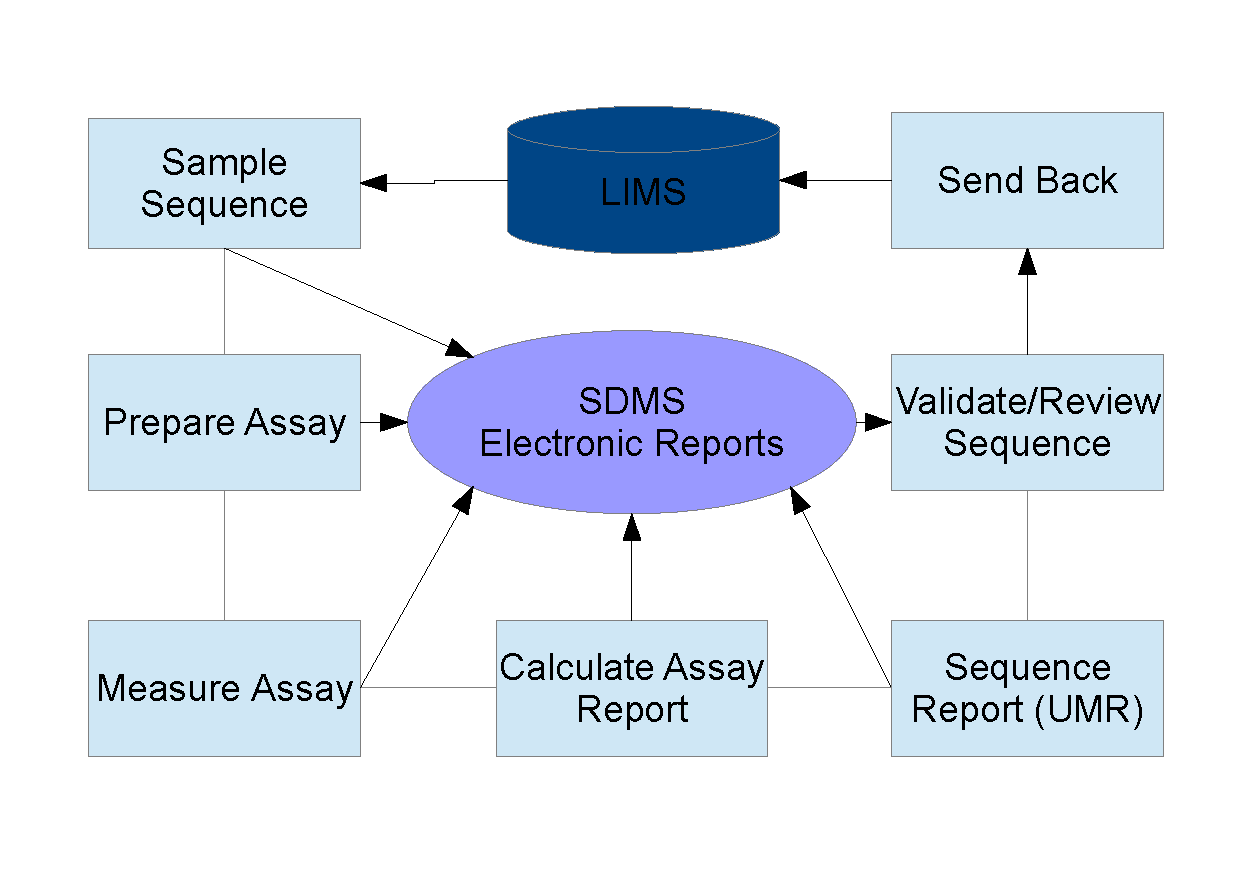
\includegraphics[width=1\textwidth]{./img/Laboverview.png}\\
    \end{center}
  \caption{Work flow of external client call process}
  \label{externClientWorkflow}
\end{figure} 



\section{Componetns}
Components are reusable functions and classes. In java the classes are put together in a jar file. These jar files can be imported in an other 
project and so be easyly used.
Jar files can be tested separately and be provided in an maven repository.

For this project a few of these componetns where created. For one they would have at some point been needed anyway and for the other reason to 
demonstrate the workflow with the buildtools and repositorys.


\subsection{Marshalling}


\subsection{Compression}



\subsection{excel adapter}






\section{Build tools}
The question what build tool, if any, came pretty early in the project development. Just starting a Project in Eclipse i the easiest way. 
At least as long as the project is not to big, is only one project and doesn't really change over time. That was all not the case. So lets have a look at few of them. 

In the Java World there are the usual suspects:
\begin{itemize}
 \item Ant
 \item Maven
 \item Gradle
\end{itemize}

\subsection{Ant}
Ant is the oldest of the three. It allows to define build scripts in xml. 
It has no own logic, so all tasks or targets have to be written from scratch.
That allows a big flexibility, it is however also quit complex. There is also the fact,
that scripting in xml is not really fun.


\subsection{Maven}
Maven also uses also xml for the configuration. Opposed to ant, you define how the project has to be build. The building is then
made by maven. Maven also resolves dependency. Maven is widely used and therefore has a lot of plugins and additional tools like an eclipse plugin. For our case maven seemed to do the job.


\subsection{Gradle}
Gradle is the newes member in the build tool family. Gradle is not just a Java build tool so i can also handle other languages. The configuration file is writen in groovy. That makes a much nicer looking project definition.
Gradle also doesn't reinvent the world. It uses the same dependency resolvement as maven. So it can almost do everything that maven can. In addition, it is easy to create custom tasks like in ant.

The downside is, that gradle is still a very young project and has not as much plugins or examples as maven. It is however worth keeping in sight.

\subsection{Usage}
For the main Webapplicatin it is the simples way to use maven as the buildtool. Since gradle seems very promissing, the plan is to use it in the smaler subprojects. That way it can be easily evaluated and maybe used as the main buildtool in the future.


\section{Testing}

\section{Versioning}
For the versioning of the source code there are several producs available. Just to name a few of them: svn, mercurial, git.
During the development of the example git was already used. It is has decentral achitecture. So every developer has always the full power of git at his disposal. It is also easy to create branches and to create labels for realases.

\subsection{using git}
In order that every user uses the branches the same way, a vew ground rules have to be set.
Each git repo will have at leas three branches. productive, validation, and master.

Master is always the newes development branch. When the new feature is ready the changes are merged into the validation branch where they are tested. This validation branch gets the name of the new version.
The only thing that has to be changed in the application configuration, is the database configuration in the spring context files.
The same has to be done when the productive package is about to be build. Since the configuration for the validation and productive 
environment can be in a separate file, the change is minimal. Only some imports have to be changed.




%FIXME do some drawings



\section{Deployment}

maven + repo + scripts + gradle


\section{Infrastructure}
This chapter shal give an overview how the infrastrucure that supports the webapp and the development of it, has to look. 
All named server are planed to be virtual machines.

It would have four servers. 
\begin{itemize}
 \item Webapplicatin server
 \item Database server
 \item Calculation server (excel, r)
 \item Repository server
\end{itemize}

\subsection{Webbapplication server}
This server is a classic webapplication server that can run war Archives. 
So it runs an jee enviroment like jBoss or tomcat.
The operating system is therefore not so relevant. 

To keep things simpel linux was choosen for the example server.

\subsubsection{configuration}
%configs....


\subsection{Database server}
De database server would be used to store the activiti data. The databases supported by activiti are mysql, oracle. Mssql is jet in experimental state.
 
For the example a linux server with a mysql database was setup.
To manage the database phpmyadmin is used.

Since the database is configured in the webapplication with spring, it is very easy to change the used database.


\subsection{Calculation server}
This is a rahter exotic configuration. This server should be able to run excel. Therefore windows is the only option al the operating system. On this server there will also run the calculation server (java) wich listens to the querrys of an activiti task.



\subsection{Repository server}
This server would not be used in the productiv setting. It is just there to facilitate the developers work.
The server would provide a maven repository and a git repository. 

The operating system would be preferably linux. That is because git is native to linux.
For the maven repository nexus from (xxxx) would be a nice chois. It supports all neccesery functions and provides a nice web frontend for managing the repositoris.

% see chapter? configuration....






\section{Migration}


\section{Data}





\addcontentsline{toc}{section}{Literaturverzeichnis}
\begin{thebibliography}{99}

\bibitem{middleware} \url{wiki}

\bibitem{activiti} \url{http://www.activiti.org/}

\bibitem{omg} \url{http://www.omg.org/}

\bibitem{eclipse} \url{http://www.eclipse.org} %FIXME

\bibitem{vaadin} \url{http://www.vaadin.com}

\bibitem{ant} \url{http://www.vaadin.com}

\bibitem{maven} \url{http://www.vaadin.com}

\bibitem{gradle} \url{http://www.vaadin.com}

\bibitem{spring} \url{} % FIXME


\bibitem{activitiDbSupport} \url{}

\bibitem{mysql} \url{}

\bibitem{phpmyadmin} \url{}

\bibitem{oracledb} \url{}

\bibitem{mssql} \url{}

\bibitem{nexus} \url{}

\bibitem{git} \url{}



\end{thebibliography}

\end{document}

